\documentclass[12pt, twoside]{article}
\usepackage[francais]{babel}
\usepackage[T1]{fontenc}
\usepackage[latin1]{inputenc}
\usepackage[left=7mm, right=7mm, top=7mm, bottom=7mm]{geometry}
\usepackage{float}
\usepackage{graphicx}
\usepackage{array}
\usepackage{multirow}
\usepackage{amsmath,amssymb,mathrsfs}
\usepackage{soul}
\usepackage{textcomp}
\usepackage{eurosym}
 \usepackage{variations}
\usepackage{tabvar}

\begin{document}


\section*{\center{Aide individualis�e: Fonctions affines}}

\subsection*{Exercice 1}

\begin{center}
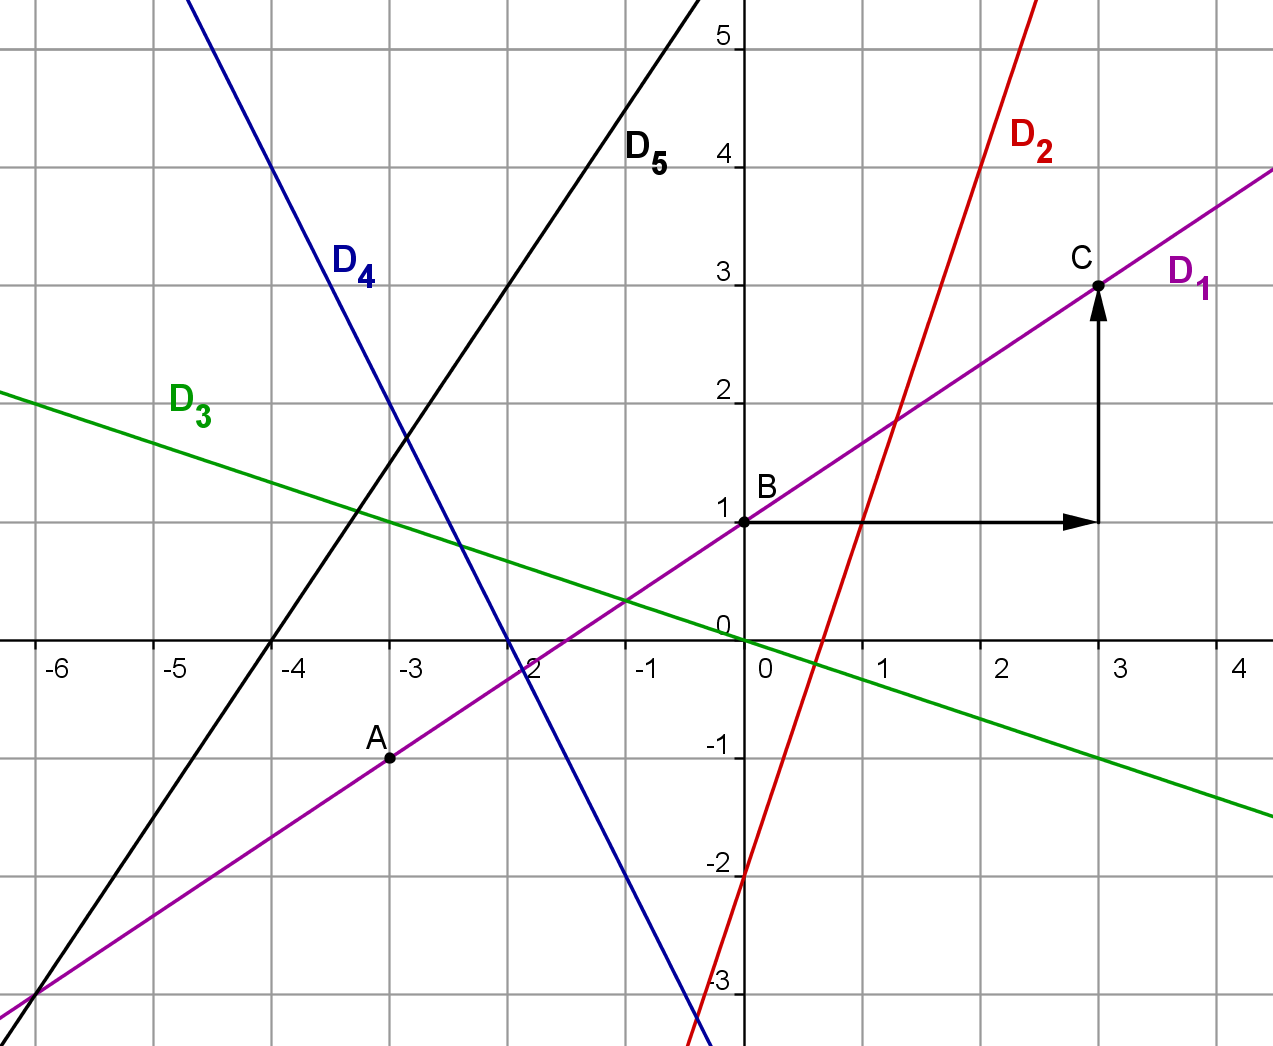
\includegraphics[width=12cm]{images/ex1.png}
\end{center}

\bigskip

Ces droites repr�sentent une fonction affine. Cette fonction s'�crit
$f(x)=ax+b$. Pour d�terminer la fonction repr�sent�e, il faut donc trouver $a$
et $b$.

\bigskip

\ul{\textbf{M�thode pour trouver a}}: $a$ est le coefficient directeur.

\enskip

\ul{Propri�t�}: Si une fonction est affine, l'accroissement de l'image est
proportionnel � l'accroissement de la variable.
Quelque
soient les r�els $x_A$ et $x_B$ (avec $x_A\neq x_B$), on a:

\begin{center}
\fbox{
$\dfrac{f(x_B)-f(x_A)}{x_B-x_A}=\dfrac{\Delta_y}{\Delta_x}=\dfrac{\text{``ce
dont je monte''}}{\text{''ce dont j'avance''}}=a$}
\end{center}


\ul{Exemple}: pour $D_1$

Je choisis 2 points de la droite qui co�ncident avec le
quadrillage, par exemple $B$ et $C$.

\begin{enumerate}
 \item $B$ a pour coordonn�es (\ldots; \ldots), $C$ a pour coordonn�es (\ldots;
\ldots).
\item  D'apr�s la formule pr�c�dente:
$a=\dfrac{f(x_C)-f(x_B)}{x_C-x_B}=\dfrac{\ldots \ldots \ldots}{\ldots \ldots
\ldots}=\dfrac{\ldots \ldots}{\ldots}$.
\item Je peux aussi trouver $a$ graphiquement: 

la diff�rence des ordonn�es  $f(x_C)-f(x_B)$ se lit avec la fl�che \ldots
\ldots \ldots \ldots, ici elle vaut \ldots \ldots

la diff�rence des abscisses $x_C-x_B$ se lit avec la fl�che \ldots \ldots
\ldots \ldots, ici elle vaut \ldots \ldots

On trouve alors $a=\dfrac{\ldots}{\ldots}$=\ldots

\pagebreak

\item Lire graphiquement le coefficient directeur $a$ en utilisant les points
$A$ et $B$. Que remarque t-on?
\end{enumerate}

\bigskip

\ul{\textbf{M�thode 1 pour trouver b}}: $b$ est appel� l'ordonn�e � l'origine
cela signifie que $b$ est l'image de $0$ par $f$.

On peut �crire de fa�on �quivalente:

$f(\ldots)=\ldots$

le point (\ldots; \ldots) appartient � la courbe repr�sentative de $f$.

\enskip

\ul{Exemple}: pour $D_1$


$b=\ldots$

on en d�duit que $f_1(x)=$\ldots\ldots\ldots\ldots

\bigskip

\ul{\textbf{M�thode 2 pour trouver b}}: Il suffit d'avoir un point de la courbe
pour d�terminer $b$. 

\enskip

\ul{Exemple}: pour $D_1$ 

Pr�c�demment nous avions choisi le point $B$ qui est le point d'intersection de
la courbe et de l'axe des ordonn�es. Parfois, il n'est pas visible. Utilisons
cette fois le point $A$.

\enskip

$A$ a pour coordonn�es (\ldots; \ldots) cela signifie que $f_1(\ldots)=\ldots$.


Je connais d�j� $a$, je peux donc remplacer dans $f_1$: $f_1(\ldots)= \ldots
\times \ldots +b$. 

J' en d�duis: \ldots=\ldots $\times $ \ldots $+b$, on a donc $b=\ldots$.

Finalement $f_1(x)=\ldots\ldots\ldots\ldots$ 

\bigskip

\textbf{D�terminer par la m�thodes de votre choix l'expression des fonctions
repr�sent�s sur le graphique.} 

\bigskip

\bigskip

\bigskip



\subsection*{Exercice 2}

Tracer la repr�sentation graphique des fonctions suivantes:
\begin{enumerate}
  \item $f(x)=2/5x+3$
  \item $g(x)=-1/3x-1$
  \item $h(x)=4x+2$
\end{enumerate}
 
\begin{center}
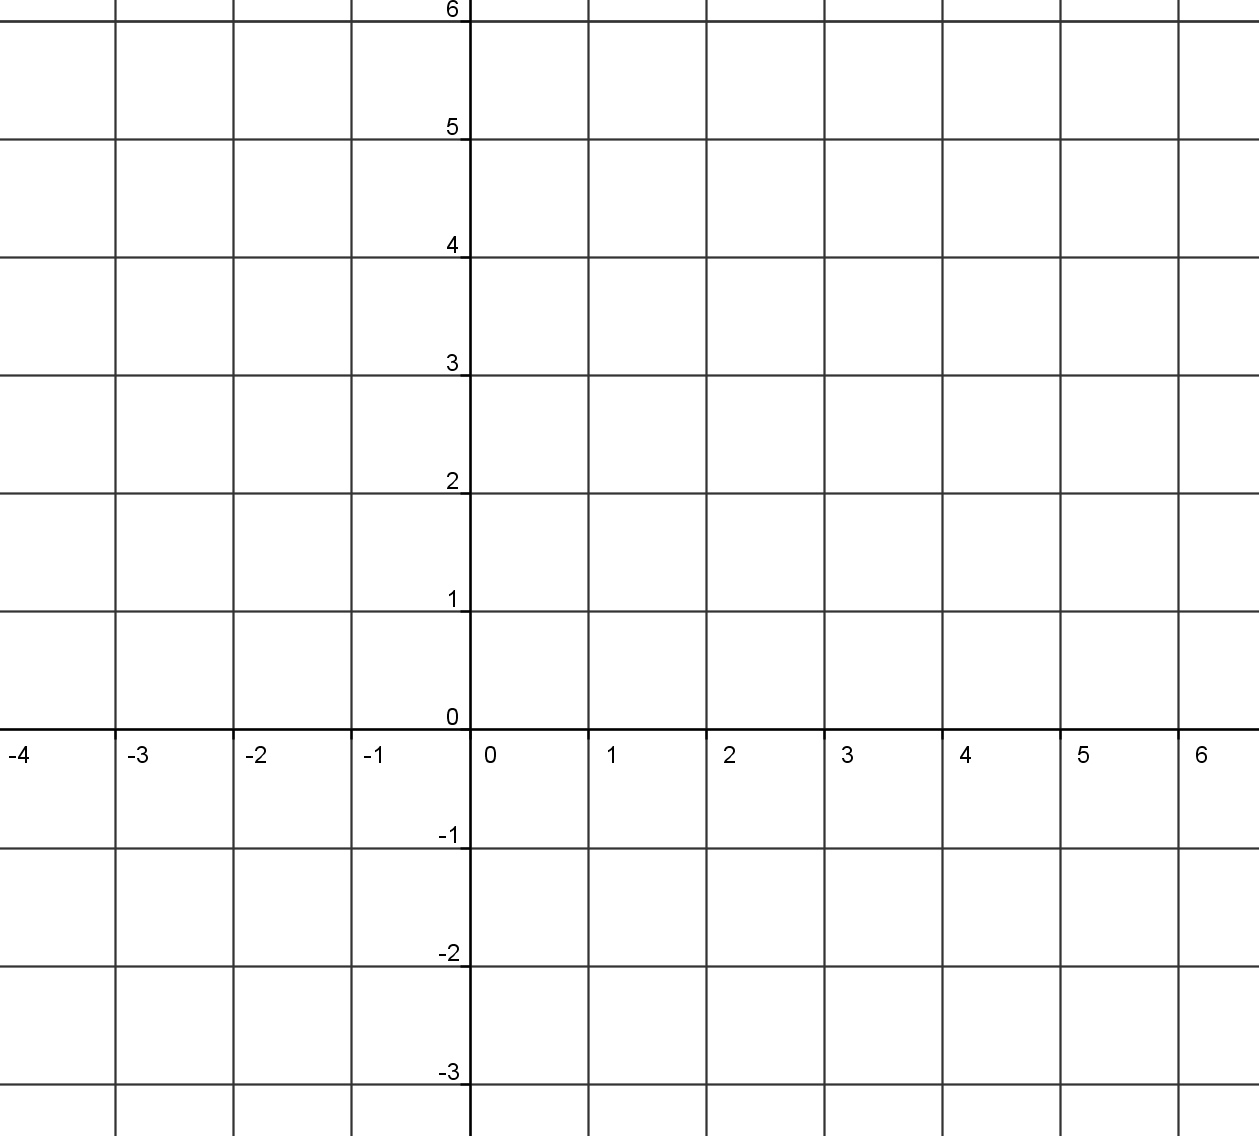
\includegraphics[width=10cm]{images/ex2.png}
\end{center}


\end{document}
